%=====================================================================
\section{Consecutive squares}\label{sec:squares}
%=====================================================================
Squares are the first nonlinear sequence after the integers, and the graph is built from squares $(N+1)^2$. We first record an elementary bound and then determine the exact supremum.

\begin{lemma}[Elementary route]\label{lem:sq8}
For $n\ge2$, $n^2\xrightarrow{-(n-1)}n-1$ and $n\xrightarrow{+n}(n+1)^2$ are legal moves. Hence $\dist(n^2,(n+1)^2)\le2+\dist(n-1,n)\le8$. For $n=1$, $1\xrightarrow{+1}4$.
\end{lemma}
\begin{proof} $(N+1)^2=n^2$ divides $n^2$ and $n^2(n-1)/n^2=n-1$, so $-(n-1)$ is legal at $n^2$; and $n\mid n$ with $n(n+1)^2/n=(n+1)^2$. Combine with Theorem~\ref{thm:successor}. \end{proof}

\begin{theorem}[Consecutive squares]\label{thm:squares}
$\dist(n^2,(n+1)^2)\le5$ for every $n\ge1$, and $\dist(23^2,24^2)=5$. Hence
\[\sup_{n\ge1}\dist(n^2,(n+1)^2)=5.\]
\end{theorem}
\noindent\emph{Source.} The bound, the 24 path identities and the lower bound at $n=23$ are from U2-SQ~\cite{u2sq}; they are re-derived and re-checked here.

\subsection{Upper bound: 24 identities}
Write $n=24t+r$, $0\le r<24$. Appendix~\ref{app:sq} lists, for each $r$, at most five signed labels $N_1(t),\dots,N_\ell(t)$ ($\ell\le5$) that carry $n^2$ to $(n+1)^2$, with all intermediate states and cofactors.
\begin{proposition}[Square identities]\label{prop:sqid}
For each $r\in\{0,\dots,23\}$ and every $t\ge t_0(r)$ (with $t_0=1$ for $r\in\{0,1,2,3\}$ and $t_0=0$ otherwise) the labelled route of Table~\ref{tab:sq} starting at $n^2$ is legal and ends at $(n+1)^2$. \emph{(Certified, Lemma~\ref{lem:certificate}.)}
\end{proposition}
\begin{example}[Class $r=1$]\label{ex:sq1}
For $n=24t+1$ (so $n+1=2(12t+1)$):
\begin{align*}
n^2&\xrightarrow{+n^2}(n^2+1)^2=4(288t^2+24t+1)^2 \\
&\xrightarrow{-24t(12t+1)}96t(12t+1)
\xrightarrow{+6t}16(12t+1)(6t+1)^2\\
&\xrightarrow{-(12t+1)}4(12t+1)^2=(n+1)^2,
\end{align*}
with cofactors $1,\,4,\,16(12t+1),\,4(12t+1)$. The first step is $x\mapsto(x+1)^2$ at $x=n^2$ (the edge with $N=x$, $k=1$); the second uses $N+1=24t(12t+1)+1=288t^2+24t+1$.
\end{example}
\begin{example}[The sharp instance $n=23$]\label{ex:23}
Class $r=23$, $t=0$: $529\xrightarrow{+1}2116\xrightarrow{+2}9522\xrightarrow{-68}136\xrightarrow{+17}2592\xrightarrow{-2}576$, of length five (Figure~\ref{fig:worked}).
\end{example}
\begin{lemma}[Coverage]\label{lem:sqcover}
Every $n\ge1$ lies in a class with $t\ge t_0$, except $n=1,2,3$, for which the routes $1\to4$ (moves $+1$), $4\to16\to100\to9$ (moves $+1,+4,-9$) and $9\to100\to16$ (moves $+9,-4$) have lengths $1,3,2$.
\end{lemma}
\begin{proof} The residues $r\ge4$ and $r=0$ cover all $n\ge4$ with $t\ge t_0$; for $r\in\{1,2,3\}$ the exclusion $t=0$ is exactly $n\in\{1,2,3\}$ (for $r=0$, $t\ge1$ means $n\ge24$, and $n=0$ is not a vertex). The three exceptional routes: $16=4\cdot4$, $16\to100$ by $16=4\cdot4$, $+4$ with $4\cdot25$; $100=10^2\to9$ by $-9$; $9\to100$ by $+9$, and $100\to16$ by $-4$ ($100=4\cdot5^2$). \end{proof}

\subsection{Lower bound}
\begin{proposition}\label{prop:23}
$\dist(23^2,24^2)=5$.
\end{proposition}
\begin{proof} Example~\ref{ex:23} gives $\le5$. The balls $\Ball_2(529)$ and $\Ball_2(576)$ have $97$ and $562$ vertices and are disjoint (\emph{computed}), so $\dist>4$ by Lemma~\ref{lem:mitm}. \end{proof}
\emph{Proof of Theorem~\ref{thm:squares}.} Proposition~\ref{prop:sqid}, Lemma~\ref{lem:sqcover} and Proposition~\ref{prop:23}. \hfill$\square$

\subsection{Distribution and remarks}
For $n\le150$ the exact distances $\dist(n^2,(n+1)^2)$ (computed here) take the values $1,2,3,4,5$ with multiplicities $1,\ 2,\ 37,\ 89,\ 21$ and mean $3.847$; the value $5$ first occurs at $n=23,28,36,40,43,47,52,59,60,\dots$. The earlier release, which computed the table for $n\le500$, reports $94$ values of $n$ with distance $5$ (inherited). The identities of Table~\ref{tab:sq} give routes of length $4$ or $5$, which are not always shortest.
\begin{remark}
That $\dist(n^2,(n+1)^2)=5$ for infinitely many $n$ is not established. The identity lengths are only upper bounds, and a refinement of the modulus could lower them in some classes.
\end{remark}
\begin{table}[ht]\centering\small
{\footnotesize\begin{longtable}{@{}rcrp{0.7\textwidth}@{}}\toprule
$r$ & $t\ge$ & moves & labels $N_i(t)$ for $n=24t+r$\\\midrule\endhead
0 & 1 & 5 & $+(12 t),\ +(12 t),\ +1,\ -(24 t + 1),\ -(24 t + 1)$ \\
1 & 1 & 4 & $+(\left(24 t + 1\right)^{2}),\ -(24 t \left(12 t + 1\right)),\ +(6 t),\ -(12 t + 1)$ \\
2 & 1 & 4 & $-(12 t),\ +(6 t),\ -(12 t + 1),\ +(2 \left(12 t + 1\right))$ \\
3 & 1 & 4 & $+3,\ -1,\ -(8 t),\ +(6 t)$ \\
4 & 0 & 5 & $+1,\ +(2 \left(6 t + 1\right)),\ +(2 \left(6 t + 1\right)),\ -(24 t + 5),\ -(24 t + 5)$ \\
5 & 0 & 4 & $+(\left(24 t + 5\right)^{2}),\ -(12 \left(4 t + 1\right) \left(6 t + 1\right)),\ +(6 t + 1),\ -(3 \left(4 t + 1\right))$ \\
6 & 0 & 4 & $-(2 \left(6 t + 1\right)),\ +(6 t + 1),\ -(3 \left(4 t + 1\right)),\ +(6 \left(4 t + 1\right))$ \\
7 & 0 & 5 & $+1,\ +2,\ -(4 \left(18 t + 5\right)),\ +(18 t + 5),\ -2$ \\
8 & 0 & 5 & $+1,\ +1,\ -(3 \left(16 t + 5\right)),\ +(16 t + 5),\ -3$ \\
9 & 0 & 4 & $+(9 \left(8 t + 3\right)^{2}),\ -(8 \left(3 t + 1\right) \left(12 t + 5\right)),\ +(2 \left(3 t + 1\right)),\ -(12 t + 5)$ \\
10 & 0 & 4 & $-(4 \left(3 t + 1\right)),\ +(2 \left(3 t + 1\right)),\ -(12 t + 5),\ +(2 \left(12 t + 5\right))$ \\
11 & 0 & 5 & $+1,\ +2,\ -(8 \left(9 t + 4\right)),\ +(2 \left(9 t + 4\right)),\ -2$ \\
12 & 0 & 5 & $+(6 \left(2 t + 1\right)),\ +(6 \left(2 t + 1\right)),\ +1,\ -(24 t + 13),\ -(24 t + 13)$ \\
13 & 0 & 4 & $+(\left(24 t + 13\right)^{2}),\ -(12 \left(2 t + 1\right) \left(12 t + 7\right)),\ +(3 \left(2 t + 1\right)),\ -(12 t + 7)$ \\
14 & 0 & 4 & $-(6 \left(2 t + 1\right)),\ +(3 \left(2 t + 1\right)),\ -(12 t + 7),\ +(2 \left(12 t + 7\right))$ \\
15 & 0 & 4 & $+3,\ -1,\ -(4 \left(2 t + 1\right)),\ +(3 \left(2 t + 1\right))$ \\
16 & 0 & 5 & $+1,\ +(4 \left(3 t + 2\right)),\ +(4 \left(3 t + 2\right)),\ -(24 t + 17),\ -(24 t + 17)$ \\
17 & 0 & 4 & $+(\left(24 t + 17\right)^{2}),\ -(24 \left(3 t + 2\right) \left(4 t + 3\right)),\ +(2 \left(3 t + 2\right)),\ -(3 \left(4 t + 3\right))$ \\
18 & 0 & 4 & $-(4 \left(3 t + 2\right)),\ +(2 \left(3 t + 2\right)),\ -(3 \left(4 t + 3\right)),\ +(6 \left(4 t + 3\right))$ \\
19 & 0 & 5 & $+1,\ +2,\ -(8 \left(9 t + 7\right)),\ +(2 \left(9 t + 7\right)),\ -2$ \\
20 & 0 & 4 & $-(2 \left(3 t + 2\right)),\ +(3 t + 2),\ -(4 t + 3),\ +(2 \left(4 t + 3\right))$ \\
21 & 0 & 4 & $+(9 \left(8 t + 7\right)^{2}),\ -(4 \left(6 t + 5\right) \left(12 t + 11\right)),\ +(6 t + 5),\ -(12 t + 11)$ \\
22 & 0 & 4 & $-(2 \left(6 t + 5\right)),\ +(6 t + 5),\ -(12 t + 11),\ +(2 \left(12 t + 11\right))$ \\
23 & 0 & 5 & $+1,\ +2,\ -(4 \left(18 t + 17\right)),\ +(18 t + 17),\ -2$ \\
\bottomrule\end{longtable}}

\caption{The 24 square identities: labels $N_i(t)$ of the route from $n^2$ to $(n+1)^2$, $n=24t+r$. Intermediate states are in Appendix~\ref{app:sq}.}\label{tab:sq}\end{table}

%=====================================================================
\section{Cycles, girth and primes}\label{sec:cycles}
%=====================================================================
\subsection{Triangle-freeness}
\begin{theorem}[Triangle-free]\label{thm:triangle}
$G$ contains no triangle.
\end{theorem}
\noindent\emph{Source.} Triangle-freeness is proved in U3~\cite{u3}; U3-COR~\cite{u3cor} gives a self-contained symbolic proof. The proof below is given in full.
\begin{proof}
Suppose $x<y<z$ are pairwise adjacent, with edge labels $a$ (for $x\sim y$), $b$ (for $y\sim z$) and $c$ (for $x\sim z$) as in Lemma~\ref{lem:ratio}. Then $y=x\rho_a$, $z=y\rho_b$, $z=x\rho_c$, so $\rho_a\rho_b=\rho_c$, i.e.
\begin{equation}\label{eq:tri}
c\,(a+1)^2(b+1)^2=ab\,(c+1)^2.
\end{equation}
Multiplying by $c$ gives $abc\,(c+1)^2=\bigl(c(a+1)(b+1)\bigr)^2$, so $abc=\bigl(c(a+1)(b+1)/(c+1)\bigr)^2$ is the square of a rational number, and being an integer it is the square of an integer $h\ge1$. Then $h\,(c+1)=c\,(a+1)(b+1)$. Since $\gcd(c,c+1)=1$, $c\mid h$; write $h=ct$ with $t\ge1$. Then $ab=h^2/c=ct^2$ and $(a+1)(b+1)=t(c+1)$. Expanding the latter and using $ab=ct^2$,
\[
a+b=t(c+1)-1-ab=tc+t-1-ct^2=(t-1)(1-ct).
\]
Since $t\ge1$ and $c\ge1$ we have $t-1\ge0$ and $1-ct\le0$, so $a+b\le0$, contradicting $a,b\ge1$. \end{proof}
(The identity $a+b=(t-1)(1-ct)$ is checked symbolically in Section~\ref{sec:verification}; a search found no triangle through any vertex $x<10^4$.)

\subsection{Girth and odd girth}
\begin{theorem}[Girth]\label{thm:girth}
$\operatorname{girth}(G)=4$ and the odd girth of $G$ is $5$. In particular $G$ is not bipartite.
\end{theorem}
\noindent\emph{Source.} The original release U3~\cite{u3} proves triangle-freeness and odd girth $5$ (the cycle $6,24,96,784,27$) but does not state the girth. The value $\operatorname{girth}(G)=4$, witnessed by the cycle $2\!-\!8\!-\!36\!-\!9$, is from the corrected release U3-COR~\cite{u3cor}, which records that the value $5$ suggested in the assessment of U3 is false.
\begin{proof} $G$ has no loops and no multiple edges, so every cycle has length $\ge3$; by Theorem~\ref{thm:triangle} there are no cycles of length $3$. The closed walk $2\to8\to36\to9\to2$ has four distinct vertices and its edges are $\{2,8\}$ ($k=2,N=1$), $\{8,36\}$ ($k=4,N=2$), $\{36,9\}$ ($k=9,N=1$), $\{9,2\}$ ($k=1,N=2$), so the girth is $4$. The closed walk $6\to24\to96\to784\to27\to6$ has five distinct vertices and edges $\{6,24\}$ ($k=6,N=1$), $\{24,96\}$ ($k=24,N=1$), $\{96,784\}$ ($k=16,N=6$), $\{784,27\}$ ($k=1,N=27$), $\{27,6\}$ ($k=3,N=2$); it is a $5$-cycle. Since there is no $3$-cycle, the shortest odd cycle has length $5$. A graph with an odd cycle is not bipartite. \end{proof}
\begin{figure}[ht]\centering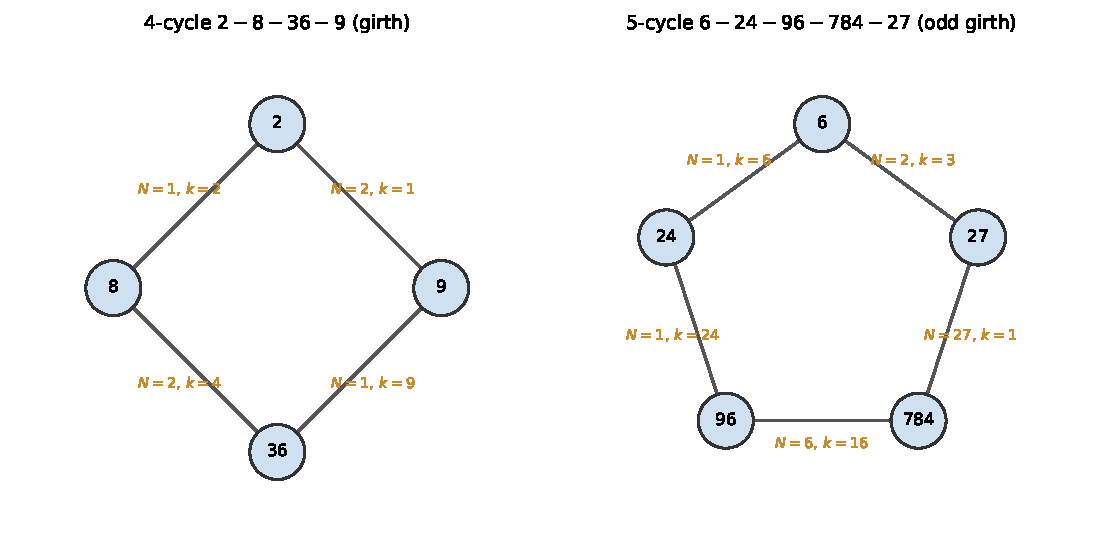
\includegraphics[width=.85\textwidth]{../figures/fig3_cycles.pdf}
\caption{The $4$-cycle and the $5$-cycle, with each edge labelled by $(N,k)$ in $\{kN,k(N+1)^2\}$.}\end{figure}
\begin{remark}[A correction]
An early assessment suggested that the girth is $5$. This is false: the cycle $2\!-\!8\!-\!36\!-\!9$ has length $4$. The correct statements, proved above, are girth $4$ and odd girth $5$; the correction was recorded in U3-COR.
\end{remark}
\begin{corollary}[Cycles through scaled vertices]\label{cor:scaledcycles}
For every $m\ge1$ the cycles $m\cdot(2,8,36,9)$ and $m\cdot(6,24,96,784,27)$ are a $4$-cycle and a $5$-cycle. In particular every even vertex lies on a $4$-cycle, and every vertex divisible by $6$ lies on both a $4$-cycle and a $5$-cycle.
\end{corollary}
\begin{proof} Theorem~\ref{thm:scaling} (scaling preserves edges and is injective). A vertex $x=2m$ equals $m\cdot2$; if $6\mid x$ then $x=(x/6)\cdot6$ lies on the scaled $5$-cycle. \end{proof}

\subsection{Primes}
By Remark~\ref{rem:primerigid} each prime $p$ has the two neighbours $4p$ and $(p+1)^2$, both composite.
\begin{theorem}[Prime distance reduction]\label{thm:primered}
For distinct primes $p,q$, $\ \dist(p,q)=2+\min\{\dist(u,v):\ u\in\{4p,(p+1)^2\},\ v\in\{4q,(q+1)^2\}\}$, and $\dist(p,q)\ge3$.
\end{theorem}
\begin{proof} $p$ and $q$ are not adjacent ($q\notin\{4p,(p+1)^2\}$ since $q$ is prime), and any path from $p$ to $q$ starts with an edge to some $u\in\Nbr(p)$ and ends with an edge from some $v\in\Nbr(q)$; the middle part has length $\ge\dist(u,v)$, and conversely a shortest $u$--$v$ path extends to a $p$--$q$ path of length $2+\dist(u,v)$. For $\dist\ge3$ we need $u\neq v$ for all choices. The equalities $4p=4q$ and $(p+1)^2=(q+1)^2$ give $p=q$; $4p=(q+1)^2$ would make $q+1$ even and $p=((q+1)/2)^2$ a perfect square, not prime; the symmetric case is the same. \end{proof}

\begin{theorem}[Certified prime distances]\label{thm:primedist}
$\dist(61,67)=7$ and $\dist(661,673)=8$.
\end{theorem}
\noindent\emph{Source.} The reduction of prime distances to distances between neighbours and the two certified values are from U2-FP~\cite{u2fp}.
\begin{proof} $61\xrightarrow{+1}244\xrightarrow{+2}1098\xrightarrow{+9}12200\xrightarrow{+488}5978025\xrightarrow{-162}36450\xrightarrow{-134}268\xrightarrow{-1}67$ has length $7$; the balls $\Ball_3(61)$ and $\Ball_3(67)$ have $322$ and $721$ vertices and are disjoint (\emph{computed}), so $\dist>6$.
$661\xrightarrow{+661}438244\xrightarrow{+2}1972098\xrightarrow{-992}1984\xrightarrow{-7}217\xrightarrow{+31}7168\xrightarrow{-3}1344\xrightarrow{+336}454276\xrightarrow{-673}673$ has length $8$; $\Ball_4(661)$ and $\Ball_3(673)$ have $123993$ and $570$ vertices and are disjoint (\emph{computed}), so $\dist>7$. \end{proof}
Consequently $6$ is not a uniform bound for consecutive primes: $673$ is the next prime after $661$ (the integers $662,\dots,672$ are composite) and $\dist(661,673)=8$. Exact distances between consecutive primes below $1200$, computed in the earlier release, take the values $4,\dots,8$; below $400$ our independent computation gives $4,\dots,7$ (Figure~\ref{fig:dist}).
\begin{figure}[ht]\centering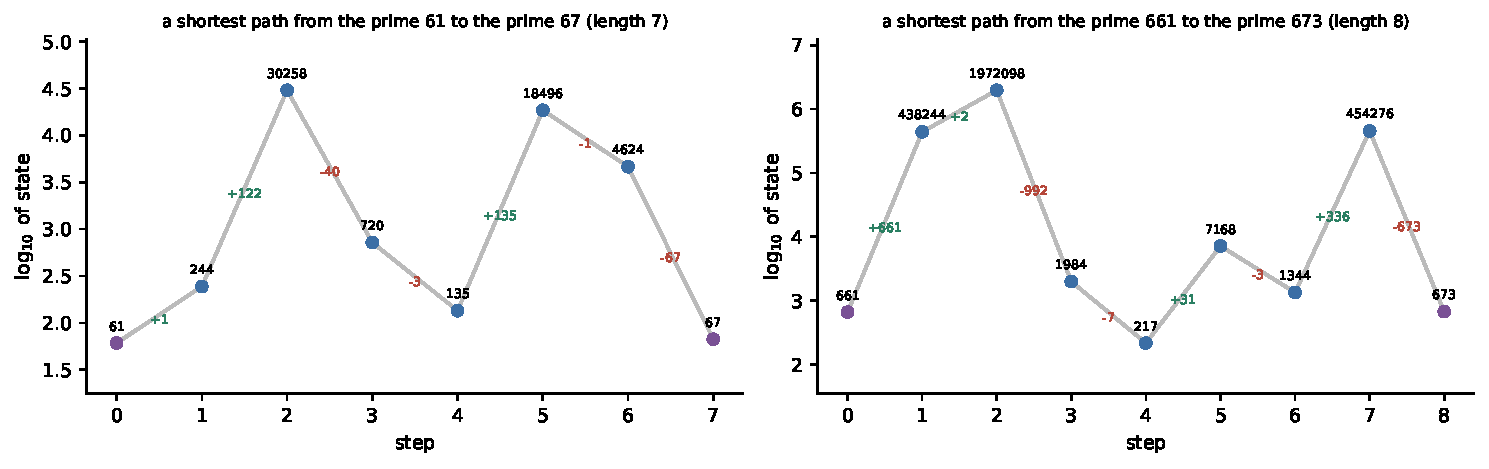
\includegraphics[width=\textwidth]{../figures/fig8_prime_paths.pdf}
\caption{Shortest paths between the primes $61$ and $67$ (length $7$) and $661$ and $673$ (length $8$). The ends are forced: from a prime one must move to $4p$ or $(p+1)^2$.}\end{figure}
